%!TEX TS-program = xelatex
\documentclass[12pt,a4paper]{report}

% --- Packages for Greek Language Support ---
\usepackage{fontspec}
\usepackage{polyglossia}
\setmainlanguage{greek}
\setotherlanguage{english}

% Set a font that supports Greek (Common on Windows/Mac/Linux)
\newfontfamily\greekfont[Script=Greek]{Times New Roman}
\newfontfamily\greekfontsf[Script=Greek]{Arial}
\newfontfamily\greekfonttt[Script=Greek]{Courier New}

% --- General Packages ---
\usepackage{geometry}
\geometry{margin=1in}
\usepackage{graphicx}
\usepackage{hyperref}
\usepackage{enumitem}
\usepackage{titlesec}
\usepackage{xcolor}
\usepackage{tikz}
\usetikzlibrary{arrows.meta, positioning, calc, shapes.geometric}
\usepackage{float}

% Custom Styling
\hypersetup{colorlinks=true, linkcolor=blue, urlcolor=blue}
\setlength{\parindent}{0pt}
\setlength{\parskip}{1em}

\tikzset{
  usecase/.style={draw, ellipse, minimum width=4.2cm, minimum height=1.0cm, align=center, fill=gray!6},
  system/.style={draw, rounded corners=8pt, minimum width=11.5cm, minimum height=8.7cm, fill=white, line width=0.9pt},
  link/.style={-{Stealth[length=2.6mm]}, thick}
}

\newcommand{\actor}[4]{%
  \begin{scope}[shift={(#1,#2)}]
    \coordinate (#4) at (0,0);
    \draw[line width=0.9pt] (0,0.28) circle (0.18);
    \draw[line width=0.9pt] (0,0.10) -- (0,-0.42);
    \draw[line width=0.9pt] (-0.24,-0.10) -- (0.24,-0.10);
    \draw[line width=0.9pt] (0,-0.42) -- (-0.20,-0.76);
    \draw[line width=0.9pt] (0,-0.42) -- (0.20,-0.76);
        \node[below=2mm] at (0,-1.25) {\small #3};
  \end{scope}
}

% --- DOCUMENT START ---
\begin{document}

% ==========================================
% TITLE PAGE
% ==========================================
\begin{titlepage}
    \centering
    
    % University Logo
    
\includegraphics[width=0.4\textwidth]{tepak-logo} % Using the actual logo in the folder
    \vspace{0.5cm}
    
    % University Info
    {\LARGE \textbf{Τεχνολογικό Πανεπιστήμιο Κύπρου}} \\[0.4cm]
    {\large \textbf{Τμήμα Μηχανικών Ηλεκτρονικών Υπολογιστών}} \\
    {\large \textbf{και Πληροφορικής}}
    
    \vspace{1.5cm}
    
    % Document Title
    \rule{\linewidth}{0.5mm} \\[0.4cm]
    {\huge \textbf{Έγγραφο Προδιαγραφών Πτυχιακής Εργασίας}}
    \rule{\linewidth}{0.5mm} \\[1cm]
    
    % Project Subject
    {\Large \textbf{Θέμα:}} \\[0.3cm]
    {\Large \textit{«CoachFlow: Διαδικτυακό Σύστημα Διαχείρισης}} \\
    {\Large \textit{Προπονητών και Πελατών»}}
    
    \vspace{1.5cm}
    
    % Supervisor Info
    {\large \textbf{Επιβλέπουσα Καθηγήτρια:}} \\
    {\large Ελίζα Αγγελίδου Λοΐζου}
    
    \vfill
    
    % Student Info (Bottom Right)
    \begin{flushright}
        \large
        \textbf{Φοιτητής:} \\
        Αντωνίου Αντρέας \\
        \textbf{ΑΦΤ:} 24892
    \end{flushright}
\end{titlepage}

% ==========================================
% TABLE OF CONTENTS
% ==========================================
\tableofcontents
\newpage

% ==========================================
% SECTION 1: ΕΙΣΑΓΩΓΗ
% ==========================================
\section{Εισαγωγή}

\subsection{Σκοπός}
Ο σκοπός αυτού του εγγράφου προδιαγραφών είναι να παρουσιάσει αναλυτικότερα την λειτουργικότητα της πλατφόρμας “CoachFlow”. Το CoachFlow είναι ένα σύγχρονο διαδικτυακό σύστημα που γεφυρώνει προπονητές (coaches) και πελάτες (clients), προσφέροντας εργαλεία για την δημιουργία και παρακολούθηση προγραμμάτων γυμναστικής (workouts), πλάνων διατροφής (nutrition), διαχείριση αγορών και επικοινωνία.

\subsection{Έκταση}
Το έγγραφο καθορίζει τις κύριες λειτουργίες του συστήματος με βάση τις απαιτήσεις των χρηστών (προπονητών και απλών χρηστών) και την αρχιτεκτονική του λογισμικού όπως αυτή έχει σχεδιαστεί και αναπτυχθεί.

\subsection{Ορισμοί}
\begin{description}
    \item[\underline{React.js, Vite, Material-UI, Bootstrap}] \hfill \\
    Οι κύριες τεχνολογίες που θα χρησιμοποιηθούν για την ανάπτυξη της διεπαφής χρήστη (Frontend). Η χρήση React επιτρέπει τη συντήρηση ενός δυναμικού και γρήγορου Single Page Application (SPA).
    
    \item[\underline{PHP, Composer, REST API}] \hfill \\
    Τεχνολογίες του Backend. Το backend διαχειρίζεται τα αιτήματα των χρηστών, επικοινωνεί με τη βάση δεδομένων και τα εξωτερικά APIs.
    
    \item[\underline{MySQL \& Firebase}] \hfill \\
    Η σχεσιακή Βάση Δεδομένων MySQL χρησιμοποιείται για την αποθήκευση των περισσότερων δεδομένων (χρήστες, προγράμματα, αγορές). Το Firebase χρησιμοποιείται για την λειτουργία ταυτοποίησης (Authentication) και συγχρονισμό δεδομένων σε πραγματικό χρόνο όπου απαιτείται.
    
    \item[\underline{Stripe API}] \hfill \\
    Η υπηρεσία που ενσωματώνεται στο σύστημα για την επεξεργασία και ασφάλεια των ηλεκτρονικών πληρωμών (συνδρομές/πακέτα προπονητών).

    \item[\underline{Mailchimp API}] \hfill \\
    Υπηρεσία marketing/email audiences που χρησιμοποιείται για εγγραφές χρηστών σε λίστες (audiences) και βασική διαχείριση campaigns όπου απαιτείται από το σύστημα.

    \item[\underline{Gmail (SMTP) / Email Service}] \hfill \\
    Υπηρεσία αποστολής transactional emails (π.χ. επιβεβαίωση εγγραφής, reset password, ειδοποιήσεις) μέσω SMTP (Gmail) από το backend.
\end{description}

\subsection{Αναφορές}

\subsubsection{Τεχνικές Ιστοσελίδες :}
\begin{itemize}[label=•]
    \item \url{https://react.dev/} (React Documentation)
    \item \url{https://mui.com/} (Material-UI)
    \item \url{https://www.php.net/} (PHP Documentation)
    \item \url{https://stripe.com/docs/} (Stripe API)
    \item \url{https://firebase.google.com/} (Firebase Setup \& Auth)
    \item \url{https://mailchimp.com/developer/} (Mailchimp Developer Docs)
\end{itemize}

\subsection{Επισκόπηση}
\begin{itemize}
    \item Στην ενότητα 2 θα γίνει παρουσίαση της αρχιτεκτονικής του συστήματος, των λειτουργιών εγγραφής/είσοδου (Authentication) και της ροής δεδομένων.
    \item Στην ενότητα 3 θα παρουσιαστούν οι κύριες οντότητες της βάσης δεδομένων (ER Diagram).
    \item Στην ενότητα 4 θα αναλυθεί η λειτουργία των πληρωμών (\textenglish{Purchases \& Subscriptions}).
    \item Στην ενότητα 5 θα παρουσιαστεί η ασφάλεια και η διαχείριση συνεδριών (Sessions/Tokens).
\end{itemize}

\newpage

% ==========================================
% SECTION 2: ΡΟΗ ΔΕΔΟΜΕΝΩΝ ΚΑΙ ΑΡΧΙΤΕΚΤΟΝΙΚΗ
% ==========================================
\section{Ροή Δεδομένων και Λειτουργίες (Features)}

\subsection{Μοντέλα Χρηστών (User Roles)}
Το σύστημα υποστηρίζει τους ακόλουθους ρόλους:
\begin{enumerate}
    \item \textbf{Επισκέπτης (Guest):} Μπορεί μόνο να εγγραφεί/συνδεθεί ή να επαναφέρει κωδικό πρόσβασης.
    \item \textbf{Αθλούμενος (Trainee):} Μπορεί να δει προπονητές, να στείλει αίτημα συνεργασίας (hire coach), να λαμβάνει/εκτελεί προγράμματα (Workout \& Nutrition) και να επικοινωνεί με τον προπονητή του.
    \item \textbf{Προπονητής (Trainer):} Μπορεί να διαχειρίζεται το προφίλ του, να αναθέτει προγράμματα στους αθλούμενους του, να παρακολουθεί την πρόοδο τους και να δέχεται πληρωμές.
    \item \textbf{Διαχειριστής (Admin):} Έχει γενική εποπτεία της πλατφόρμας, των χρηστών και των συναλλαγών (Analytics, System health).
\end{enumerate}

\subsubsection{Λειτουργίες ανά ρόλο (Functional Use Cases)}
\textbf{Trainee (Αθλούμενος)}
\begin{itemize}[label=•]
    \item \textbf{Διατροφή:} Αναζήτηση τροφών μέσω \textenglish{USDA} βάσης δεδομένων, καταγραφή γευμάτων/τροφών, προβολή ιστορικού και συνοπτικών στοιχείων (daily summaries).
    \item \textbf{Προπόνηση:} Εκκίνηση προπόνησης/προγράμματος, καταγραφή σετ/ασκήσεων, δυνατότητα \textenglish{skip} για ασκήσεις ή σετ, προβολή ιστορικού συνεδριών.
    \item \textbf{Σώμα/Μετρήσεις:} Καταγραφή βάρους και βασικών μετρήσεων (π.χ. waist), προβολή προόδου και αναλυτικών (analytics).
    \item \textbf{Προγράμματα:} Δημιουργία/επεξεργασία προσωπικών plans, αγορά plans από trainers, διαχείριση αγορών (π.χ. edit/delete/hide όπου επιτρέπεται).
    \item \textbf{Coach/Trainer σχέση:} Αποστολή αιτήματος συνεργασίας, σύνδεση/αποσύνδεση, ανταλλαγή μηνυμάτων, εκτέλεση προγραμμάτων του trainer.
    \item \textbf{Αξιολογήσεις:} Αξιολόγηση trainer και αξιολόγηση αγορασμένου workout plan.
    \item \textbf{Analytics:} Προβολή στατιστικών και φιλτράρισμα με ημερομηνίες (date ranges).
    \item \textbf{Προφίλ:} Προβολή και αλλαγή στοιχείων προφίλ.
\end{itemize}

\textbf{Trainer (Προπονητής)}
\begin{itemize}[label=•]
    \item \textbf{Προφίλ/Overview:} Προβολή επισκόπησης (dashboard), ενημέρωση προφίλ και διαθεσιμότητας.
    \item \textbf{Προγράμματα προς πώληση:} Δημιουργία custom προγραμμάτων (workout plans) για marketplace/πωλήσεις και διαχείριση αυτών.
    \item \textbf{Αιτήματα/Σχέσεις:} Προβολή και αποδοχή αιτημάτων από trainees, τερματισμός σχέσης (disconnect).
    \item \textbf{Διαχείριση trainees:} Ανάθεση προγραμμάτων, ανάθεση υπαρχόντων προγραμμάτων (re-use), παρακολούθηση προόδου/analytics.
    \item \textbf{Διατροφή trainees:} Ορισμός στόχων/πλάνων διατροφής με βάση \textenglish{USDA} ή fully custom οδηγίες ανά γεύμα/ημέρα.
    \item \textbf{Μηνύματα:} Επικοινωνία με trainees.
\end{itemize}

\textbf{Admin (Διαχειριστής)}
\begin{itemize}[label=•]
    \item \textbf{Platform analytics:} Συνολικά στατιστικά πλατφόρμας (users, purchases, activity).
    \item \textbf{User management:} Προσθήκη/επεξεργασία/διαγραφή, disable/enable, \textenglish{force reset password}.
    \item \textbf{Email marketing:} Δημιουργία campaigns (π.χ. μέσω Mailchimp) με custom HTML emails ή templates.
    \item \textbf{Μηνύματα:} Δυνατότητα επικοινωνίας με χρήστες της πλατφόρμας.
    \item \textbf{Προφίλ:} Προβολή και αλλαγή στοιχείων προφίλ.
\end{itemize}

\subsection{Διαγράμματα Χρήσης (Use Cases)}
\subsubsection{Διαγράμματα Χρήσης (Use Case Diagrams)}
\noindent 1. Account Access
% 1. Account Access (TikZ)
\begin{figure}[H]
    \centering
    \begin{tikzpicture}[font=\small]
        % System boundary
        \node[system, minimum width=12.8cm, minimum height=7.8cm] (sys) {};
        \node[anchor=west, font=\bfseries] at ($(sys.north west)+(0.35,-0.35)$) {CoachFlow - Account Access};

        % Actors
        \actor{-7.25}{ 2.75}{Guest}{guest}
        \actor{-7.25}{ 0.85}{Trainee}{trainee}
        \actor{-7.25}{-1.05}{Trainer}{trainer}
        \actor{-7.25}{-2.95}{Admin}{admin}

        % Use cases
        \node[usecase, minimum width=5.0cm] (register) at (1.85, 2.05) {Register (Sign Up)};
        \node[usecase, minimum width=4.6cm] (reset)    at (1.85, 0.75) {Reset Password};
        \node[usecase, minimum width=3.2cm] (login)    at (1.85,-0.45) {Login};
        \node[usecase, minimum width=3.2cm] (logout)   at (1.85,-1.75) {Logout};
        \node[usecase, minimum width=4.6cm] (profile)  at (1.85,-3.05) {Manage Profile};

        % Links
        \draw[link] (guest)   -- (register.west);
        \draw[link] (guest)   -- (reset.west);
        \draw[link] (guest)   -- (login.west);

        \draw[link] (trainee) -- (logout.west);
        \draw[link] (trainee) -- (profile.west);

        \draw[link] (trainer) -- (logout.west);
        \draw[link] (trainer) -- (profile.west);

        \draw[link] (admin)   -- (profile.west);
    \end{tikzpicture}

    \vspace{3mm}
    \textit{Guest users can only sign up / login / reset password. All other actions require authentication.}
\end{figure}
\clearpage

\noindent 2. Trainee-Trainer Interaction
% 2. Trainee-Trainer Interaction (TikZ)
\begin{figure}[H]
    \centering
    \begin{tikzpicture}[font=\small]
        % System boundary
        \node[system, minimum width=12.8cm, minimum height=7.8cm] (sys) {};
        \node[anchor=west, font=\bfseries] at ($(sys.north west)+(0.35,-0.35)$) {CoachFlow - Trainee / Trainer Interaction};

        % Actors
        \actor{-7.25}{ 1.35}{Trainee}{trainee}
        \actor{-7.25}{-1.65}{Trainer}{trainer}

        % Use cases
        \node[usecase, minimum width=5.4cm] (browse)   at (2.15, 2.10) {Browse \& View Trainers};
        \node[usecase, minimum width=6.4cm] (request)  at (2.15, 0.95) {Send Coaching Request (Connect)};
        \node[usecase, minimum width=4.8cm] (messages) at (2.15,-0.20) {Send / Read Messages};
        \node[usecase, minimum width=3.6cm] (rate)     at (2.15,-1.35) {Rate Trainer};
        \node[usecase, minimum width=5.4cm] (disconnect) at (2.15,-2.50) {Disconnect Relationship};
        \node[usecase, minimum width=5.8cm] (manage)   at (2.15,-3.65) {Manage Requests (accept/decline)};

        % Links
        \draw[link] (trainee) -- (browse.west);
        \draw[link] (trainee) -- (request.west);
        \draw[link] (trainee) -- (messages.west);
        \draw[link] (trainee) -- (rate.west);
        \draw[link] (trainee) -- (disconnect.west);

        \draw[link] (trainer) -- (messages.west);
        \draw[link] (trainer) -- (disconnect.west);
        \draw[link] (trainer) -- (manage.west);
    \end{tikzpicture}

    \vspace{3mm}
    \textit{Only authenticated trainees can browse trainers, hire, and message. Guests have no access to these actions.}
\end{figure}
\clearpage

\noindent 3. Training Flow
% 3. Training Flow (TikZ)
\begin{figure}[H]
    \centering
    \begin{tikzpicture}[font=\small]
        % System boundary
        \node[system, minimum width=12.8cm, minimum height=7.6cm] (sys) {};
        \node[anchor=west, font=\bfseries] at ($(sys.north west)+(0.35,-0.35)$) {CoachFlow - Training Flow};

        % Actors
        \actor{-7.25}{ 1.15}{Trainee}{trainee}
        \actor{-7.25}{-1.60}{Trainer}{trainer}

        % Use cases
        \node[usecase, minimum width=6.2cm] (create)  at (2.20, 1.95) {Create / Edit Workout Plan};
        \node[usecase, minimum width=5.8cm] (assign)  at (2.20, 0.80) {Assign Program to Trainee};
        \node[usecase, minimum width=5.0cm] (start)   at (2.20,-0.35) {Start Workout Session};
        \node[usecase, minimum width=5.2cm] (log)     at (2.20,-1.50) {Log Sets / Reps / Weights};
        \node[usecase, minimum width=4.6cm] (skip)    at (2.20,-2.65) {Skip Exercise / Set};
        \node[usecase, minimum width=5.8cm] (history) at (2.20,-3.80) {Workout History \& Progress};

        % Links
        \draw[link] (trainer) -- (create.west);
        \draw[link] (trainer) -- (assign.west);
        \draw[link] (trainer) -- (history.west);

        \draw[link] (trainee) -- (start.west);
        \draw[link] (trainee) -- (log.west);
        \draw[link] (trainee) -- (skip.west);
        \draw[link] (trainee) -- (history.west);

        % Cross-role access
        \draw[link] (trainee) -- (assign.west);
        \draw[link] (trainer) -- (log.west);
    \end{tikzpicture}

    \vspace{3mm}
    \textit{Core training flow: trainers build/assign plans and trainees execute sessions with detailed logging and history.}
\end{figure}
\clearpage

\noindent 4. Payments
% 4. Payments (TikZ)
\begin{figure}[H]
    \centering
    \begin{tikzpicture}[font=\small]
        % System boundary
        \node[system, minimum width=12.8cm, minimum height=7.8cm] (sys) {};
        \node[anchor=west, font=\bfseries] at ($(sys.north west)+(0.35,-0.35)$) {CoachFlow - Payments};

        % Actors
        \actor{-7.25}{ 1.05}{Trainee}{trainee}
        \actor{-7.25}{-1.80}{Trainer}{trainer}
        \actor{ 7.25}{-0.20}{Stripe API}{stripe}

        % Use cases
        \node[usecase, minimum width=5.4cm] (browse)  at (1.90, 1.95) {Browse Programs / Plans};
        \node[usecase, minimum width=5.0cm] (intent)  at (1.90, 0.75) {Create Payment Intent};
        \node[usecase, minimum width=5.0cm] (process) at (1.90,-0.45) {Process Card Payment};
        \node[usecase, minimum width=5.0cm] (access)  at (1.90,-1.65) {Access Purchased Plans};
        \node[usecase, minimum width=5.4cm] (manage)  at (1.90,-2.85) {Manage Purchases (hide/rate)};
        \node[usecase, minimum width=5.2cm] (publish) at (1.90,-4.05) {Publish Plans \& View Sales};

        % Links
        \draw[link] (trainee) -- (browse.west);
        \draw[link] (trainee) -- (intent.west);
        \draw[link] (trainee) -- (process.west);
        \draw[link] (trainee) -- (access.west);
        \draw[link] (trainee) -- (manage.west);

        \draw[link] (trainer) -- (publish.west);

        \draw[link] (stripe) -- (intent.east);
        \draw[link] (stripe) -- (process.east);
    \end{tikzpicture}

    \vspace{3mm}
    \textit{Payments cover plan purchases (trainee) and revenue/sales visibility (trainer) via Stripe.}
\end{figure}
\clearpage

\noindent 5. Administration
% 5. Administration (TikZ)
\begin{figure}[H]
    \centering
    \begin{tikzpicture}[font=\small]
        % System boundary
        \node[system, minimum width=12.8cm, minimum height=7.8cm] (sys) {};
        \node[anchor=west, font=\bfseries] at ($(sys.north west)+(0.35,-0.35)$) {CoachFlow - Administration};

        % Actors
        \actor{-7.25}{ 0.10}{Admin}{admin}
        \actor{ 7.25}{-0.20}{Mailchimp}{mailchimp}

        % Use cases
        \node[usecase, minimum width=6.0cm] (users)    at (1.95, 2.05) {User Management (add/edit/delete)};
        \node[usecase, minimum width=5.2cm] (disable)  at (1.95, 0.90) {Disable / Enable Users};
        \node[usecase, minimum width=4.8cm] (force)    at (1.95,-0.25) {Force Password Reset};
        \node[usecase, minimum width=4.8cm] (analytics)at (1.95,-1.40) {Platform Analytics};
        \node[usecase, minimum width=5.2cm] (campaign) at (1.95,-2.55) {Create Email Campaign};
        \node[usecase, minimum width=4.8cm] (message)  at (1.95,-3.70) {Message Any User};

        % Links
        \draw[link] (admin) -- (users.west);
        \draw[link] (admin) -- (disable.west);
        \draw[link] (admin) -- (force.west);
        \draw[link] (admin) -- (analytics.west);
        \draw[link] (admin) -- (campaign.west);
        \draw[link] (admin) -- (message.west);

        \draw[link] (mailchimp) -- (campaign.east);
    \end{tikzpicture}

    \vspace{3mm}
    \textit{Administration includes platform analytics, full user management, messaging, and email marketing campaigns.}
\end{figure}
\clearpage

\noindent 6. Nutrition \& USDA
% 6. Nutrition & USDA (TikZ)
\begin{figure}[H]
    \centering
    \begin{tikzpicture}[font=\small]
        % System boundary
        \node[system, minimum width=12.8cm, minimum height=7.8cm] (sys) {};
        \node[anchor=west, font=\bfseries] at ($(sys.north west)+(0.35,-0.35)$) {CoachFlow - Nutrition \& USDA};

        % Actors
        \actor{-7.25}{ 1.30}{Trainee}{trainee}
        \actor{-7.25}{-1.75}{Trainer}{trainer}
        \actor{ 7.25}{ 0.40}{USDA}{usda}

        % Use cases
        \node[usecase, minimum width=4.6cm] (search)  at (2.05, 2.05) {Search Foods (USDA)};
        \node[usecase, minimum width=4.6cm] (log)     at (2.05, 0.85) {Log Food / Meals};
        \node[usecase, minimum width=4.8cm] (history) at (2.05,-0.35) {View Nutrition History};
        \node[usecase, minimum width=5.4cm] (goals)   at (2.05,-1.55) {Set Custom Nutrition Goals};
        \node[usecase, minimum width=4.8cm] (weekly)  at (2.05,-2.75) {Set Weekly Meal Plan};
        \node[usecase, minimum width=4.6cm] (custom)  at (2.05,-3.95) {Create Custom Foods};

        % Links
        \draw[link] (trainee) -- (search.west);
        \draw[link] (trainee) -- (log.west);
        \draw[link] (trainee) -- (history.west);

        \draw[link] (trainer) -- (goals.west);
        \draw[link] (trainer) -- (weekly.west);
        \draw[link] (trainer) -- (custom.west);

        \draw[link] (usda) -- (search.east);
    \end{tikzpicture}

    \vspace{3mm}
    \textit{Nutrition includes USDA-based food search plus logging, history, and trainer-assigned goals/meal plans.}
\end{figure}
\clearpage

\noindent 7. Analytics \& History
% 7. Analytics & History (TikZ)
\begin{figure}[H]
    \centering
    \begin{tikzpicture}[font=\small]
        % System boundary
        \node[system, minimum width=12.8cm, minimum height=7.6cm] (sys) {};
        \node[anchor=west, font=\bfseries] at ($(sys.north west)+(0.35,-0.35)$) {CoachFlow - Analytics \& History};

        % Actors
        \actor{-7.25}{ 2.35}{Trainee}{trainee}
        \actor{-7.25}{ 0.25}{Trainer}{trainer}
        \actor{-7.25}{-2.00}{Admin}{admin}

        % Use cases
        \node[usecase, minimum width=5.2cm] (personal) at (2.05, 1.85) {View Personal Analytics};
        \node[usecase, minimum width=4.8cm] (filter)   at (2.05, 0.75) {Filter by Date Range};
        \node[usecase, minimum width=4.8cm] (history)  at (2.05,-0.35) {Workout \& Food History};
        \node[usecase, minimum width=4.8cm] (log)      at (2.05,-1.45) {Log Weight / Measurements};
        \node[usecase, minimum width=4.8cm] (traineeA) at (2.05,-2.55) {View Trainee Analytics};
        \node[usecase, minimum width=4.8cm] (platform) at (2.05,-3.65) {View Platform Analytics};

        % Links
        \draw[link] (trainee) -- (personal.west);
        \draw[link] (trainee) -- (filter.west);
        \draw[link] (trainee) -- (history.west);
        \draw[link] (trainee) -- (log.west);

        \draw[link] (trainer) -- (filter.west);
        \draw[link] (trainer) -- (traineeA.west);

        \draw[link] (admin) -- (platform.west);
    \end{tikzpicture}

    \vspace{3mm}
    \textit{Users can view analytics and history with date filters; trainers see trainee analytics; admins see platform analytics.}
\end{figure}
\clearpage

Η ταυτοποίηση χρηστών (Authentication) πραγματοποιείται με τη βοήθεια του Firebase Auth, παρέχοντας ένα ασφαλές και κρυπτογραφημένο περιβάλλον. Αφού ο χρήστης ταυτοποιηθεί με επιτυχία στο Firebase, το σύστημα επικοινωνεί με το PHP backend του ελέγχοντας τα στοιχεία από τη MySQL βάση δεδομένων και επιστρέφει το αντίστοιχο προφίλ μαζί με το ρόλο του (Authority/Role).

\subsection{Αρχιτεκτονική Εφαρμογής (Class/Component Diagram)}
\subsubsection{Διαχωρισμός Frontend \& Backend :}

\begin{figure}[htbp]
    \centering
    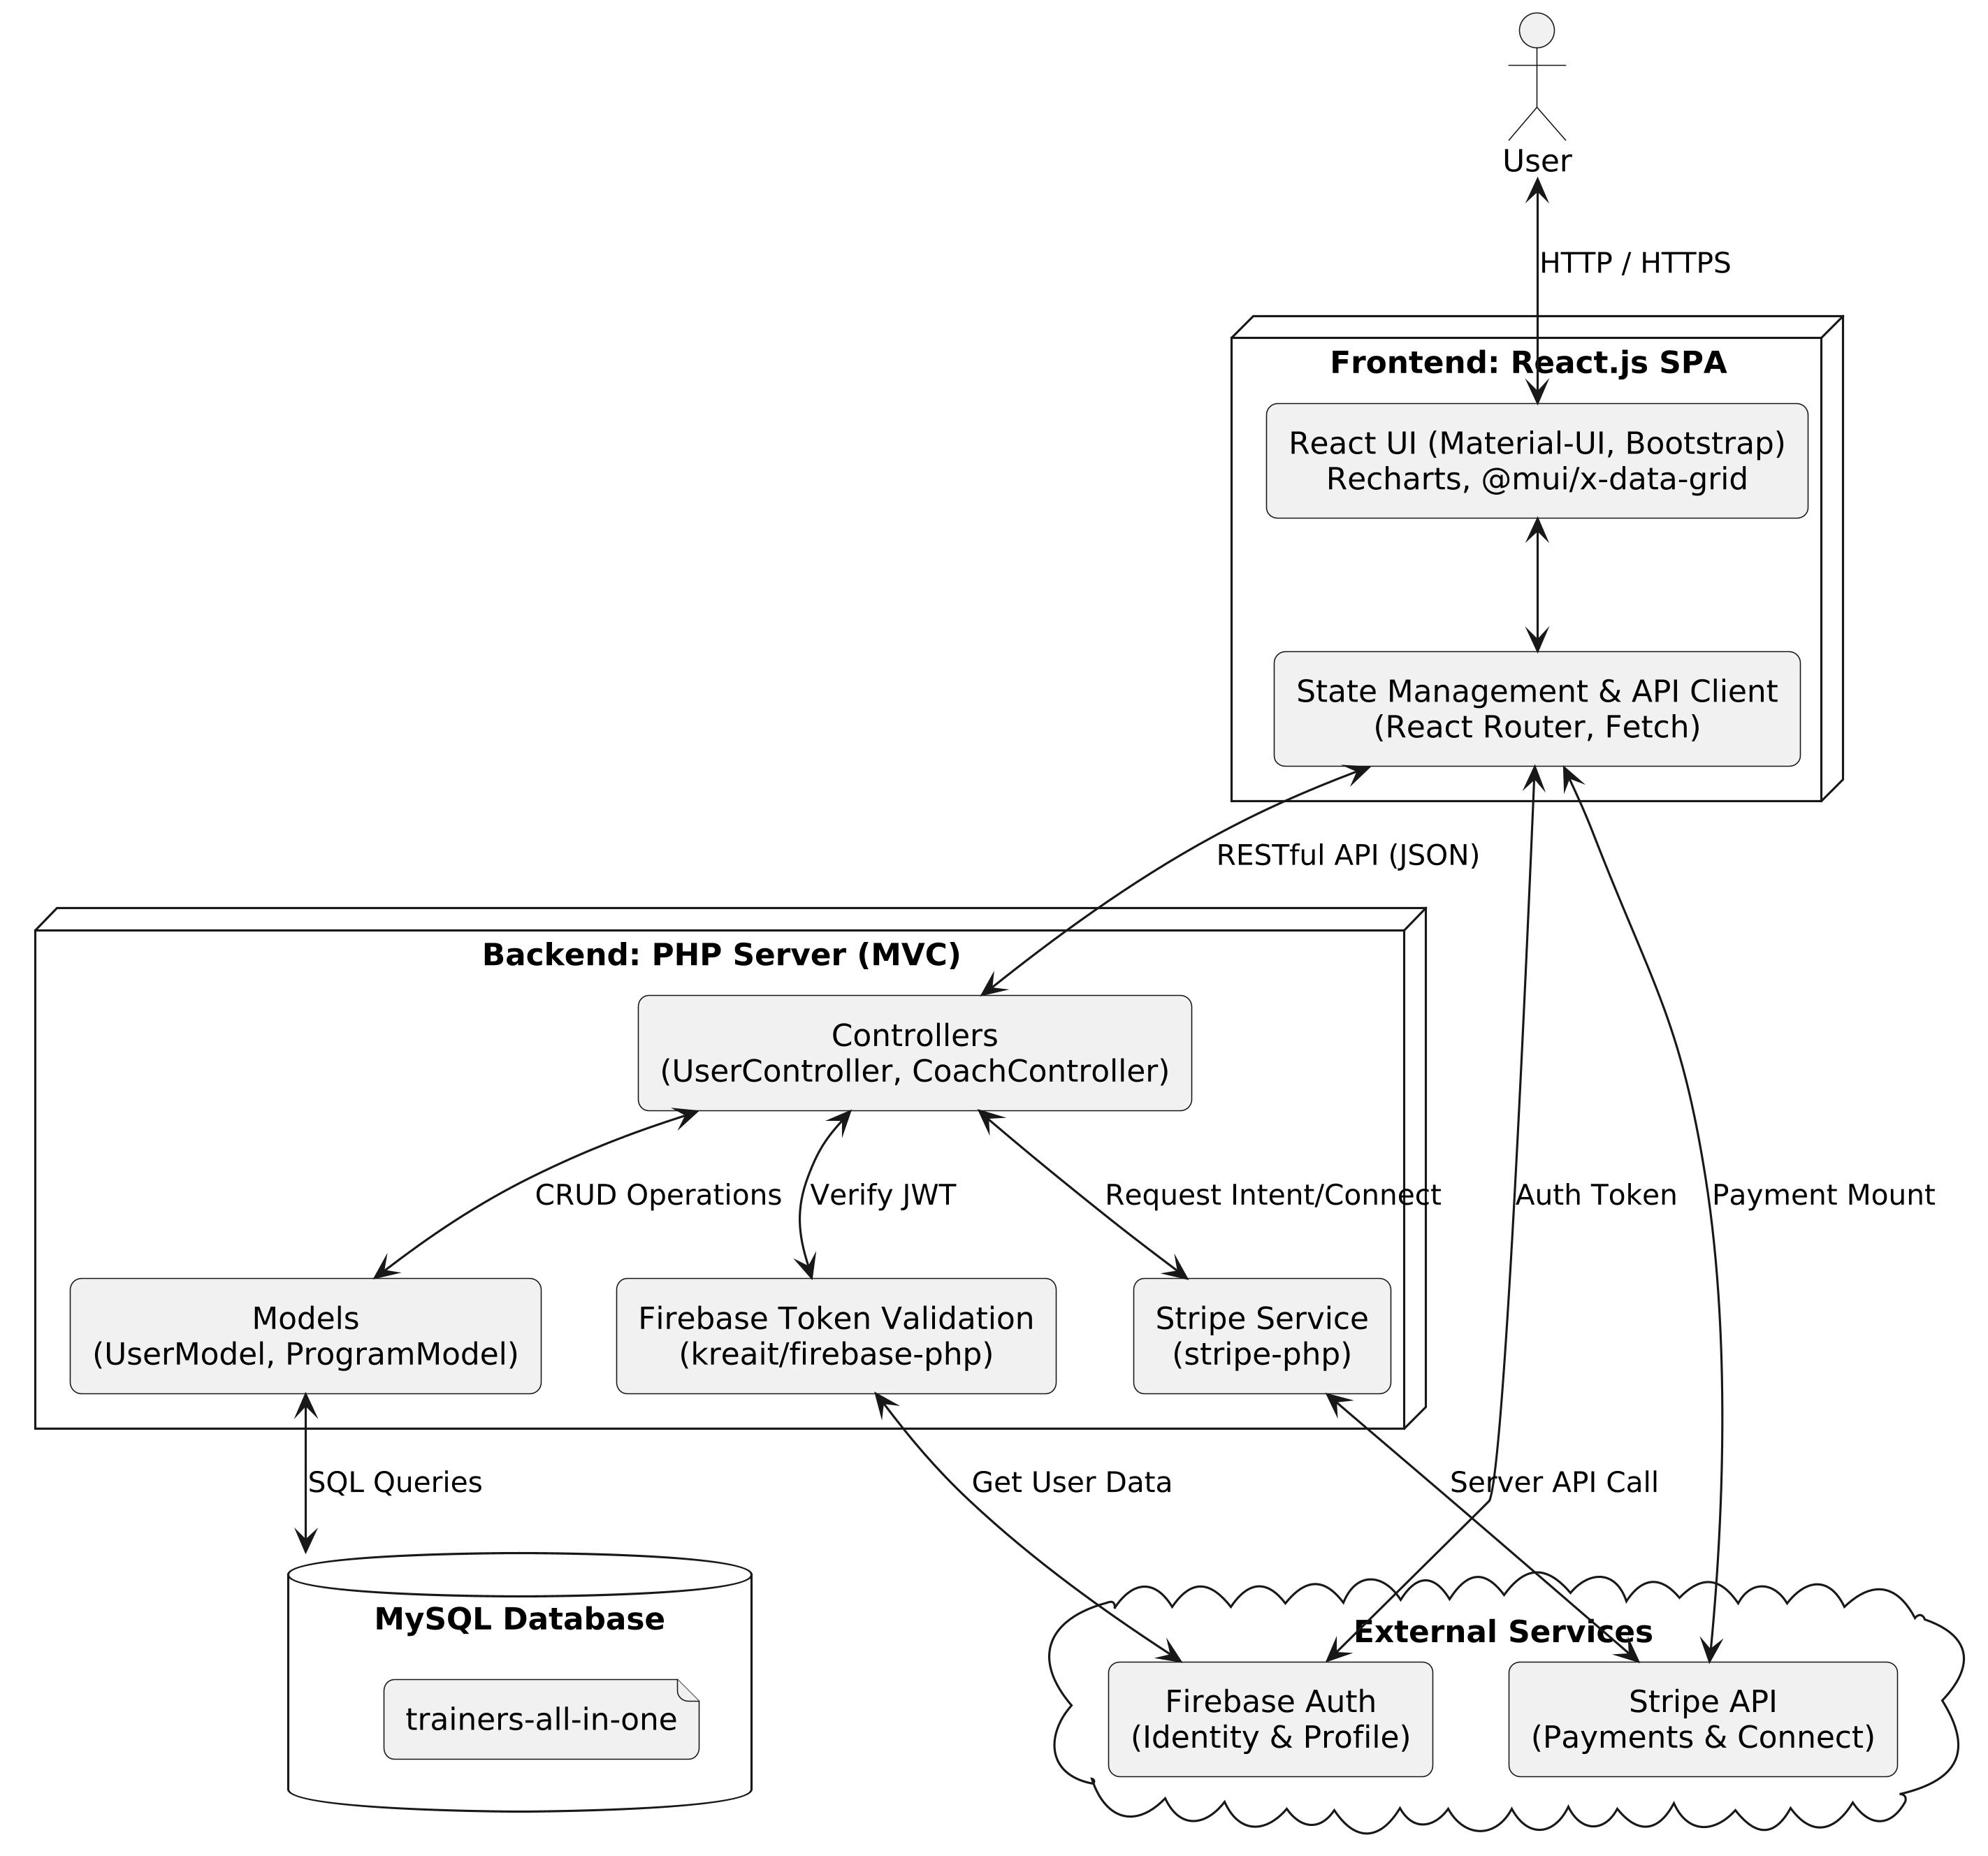
\includegraphics[width=0.9\textwidth]{arch_diagram.png}
    \caption{Architecture Diagram: SPA \& REST API Μεθοδολογία}
\end{figure}

Το σύστημα του CoachFlow ακολουθεί μια πλήρως διαχωρισμένη (decoupled) αρχιτεκτονική, αποτελούμενη από 2 βασικά υποσυστήματα. Το \textbf{Frontend Application} (React.js SPA) καταναλώνει πόρους μέσω δομημένων κλήσεων \textbf{REST API}, και ο \textbf{Backend PHP Server} λειτουργεί ως πάροχος αυτών των υπηρεσιών βασισμένος στο αρχιτεκτονικό πρότυπο Model-View-Controller (MVC).

Η διάδραση και διαχείριση της επιχειρηματικής λογικής χωρίζεται στα εξής επίπεδα:
\begin{itemize}
    \item \textbf{Frontend (React \& Vite):} Διαχειρίζεται την κατάσταση (state) και τη διεπαφή του χρήστη με την χρήση βιβλιοθηκών όπως το Material-UI για τα UI components, το Recharts για τα γραφήματα αναλυτικών στοιχείων (Analytics), και το \textenglish{@stripe/react-stripe-js} για την ασφαλή εισαγωγή καρτών. 
    \item \textbf{Controllers (PHP):} Υποδέχονται τα \textenglish{HTTP Requests} της React εφαρμογής και κατευθύνουν τη λογική του \textenglish{backend} (π.χ. \textenglish{UserController, CoachController, WorkoutController, NutritionController}). Φροντίζουν για το validation των δεδομένων προορίζοντας τα κατάλληλα HTTP Status Codes πίσω στον client.
    \item \textbf{Models (PHP) \& MySQL:} Τα Models (όπως \textenglish{UserModel, ProgramModel, PurchaseModel, AnalyticsModel}) είναι υπεύθυνα για τις εντολές SQL (Queries) και την ενσωμάτωση των δεδομένων στη σχεσιακή βάση \textenglish{trainers-all-in-one}.
    \item \textbf{Εξωτερικά Services \& Middlewares:} Το σύστημα ενσωματώνει \textenglish{Firebase Admin SDK (kreait/firebase-php)} για ασφαλή ταυτοποίηση χρηστών (JWT Validation) και το \textenglish{Stripe API} για τη διαχείριση οικονομικών συναλλαγών (Payments \& Payouts).
\end{itemize}

\newpage

% ==========================================
% SECTION 3: ΒΑΣΗ ΔΕΔΟΜΕΝΩΝ (ERD)
% ==========================================
\section{Entity - Relationship Configuration}
\subsection{Στοιχεία Βάσης Δεδομένων}

    \begin{figure}[htbp]
        \centering
        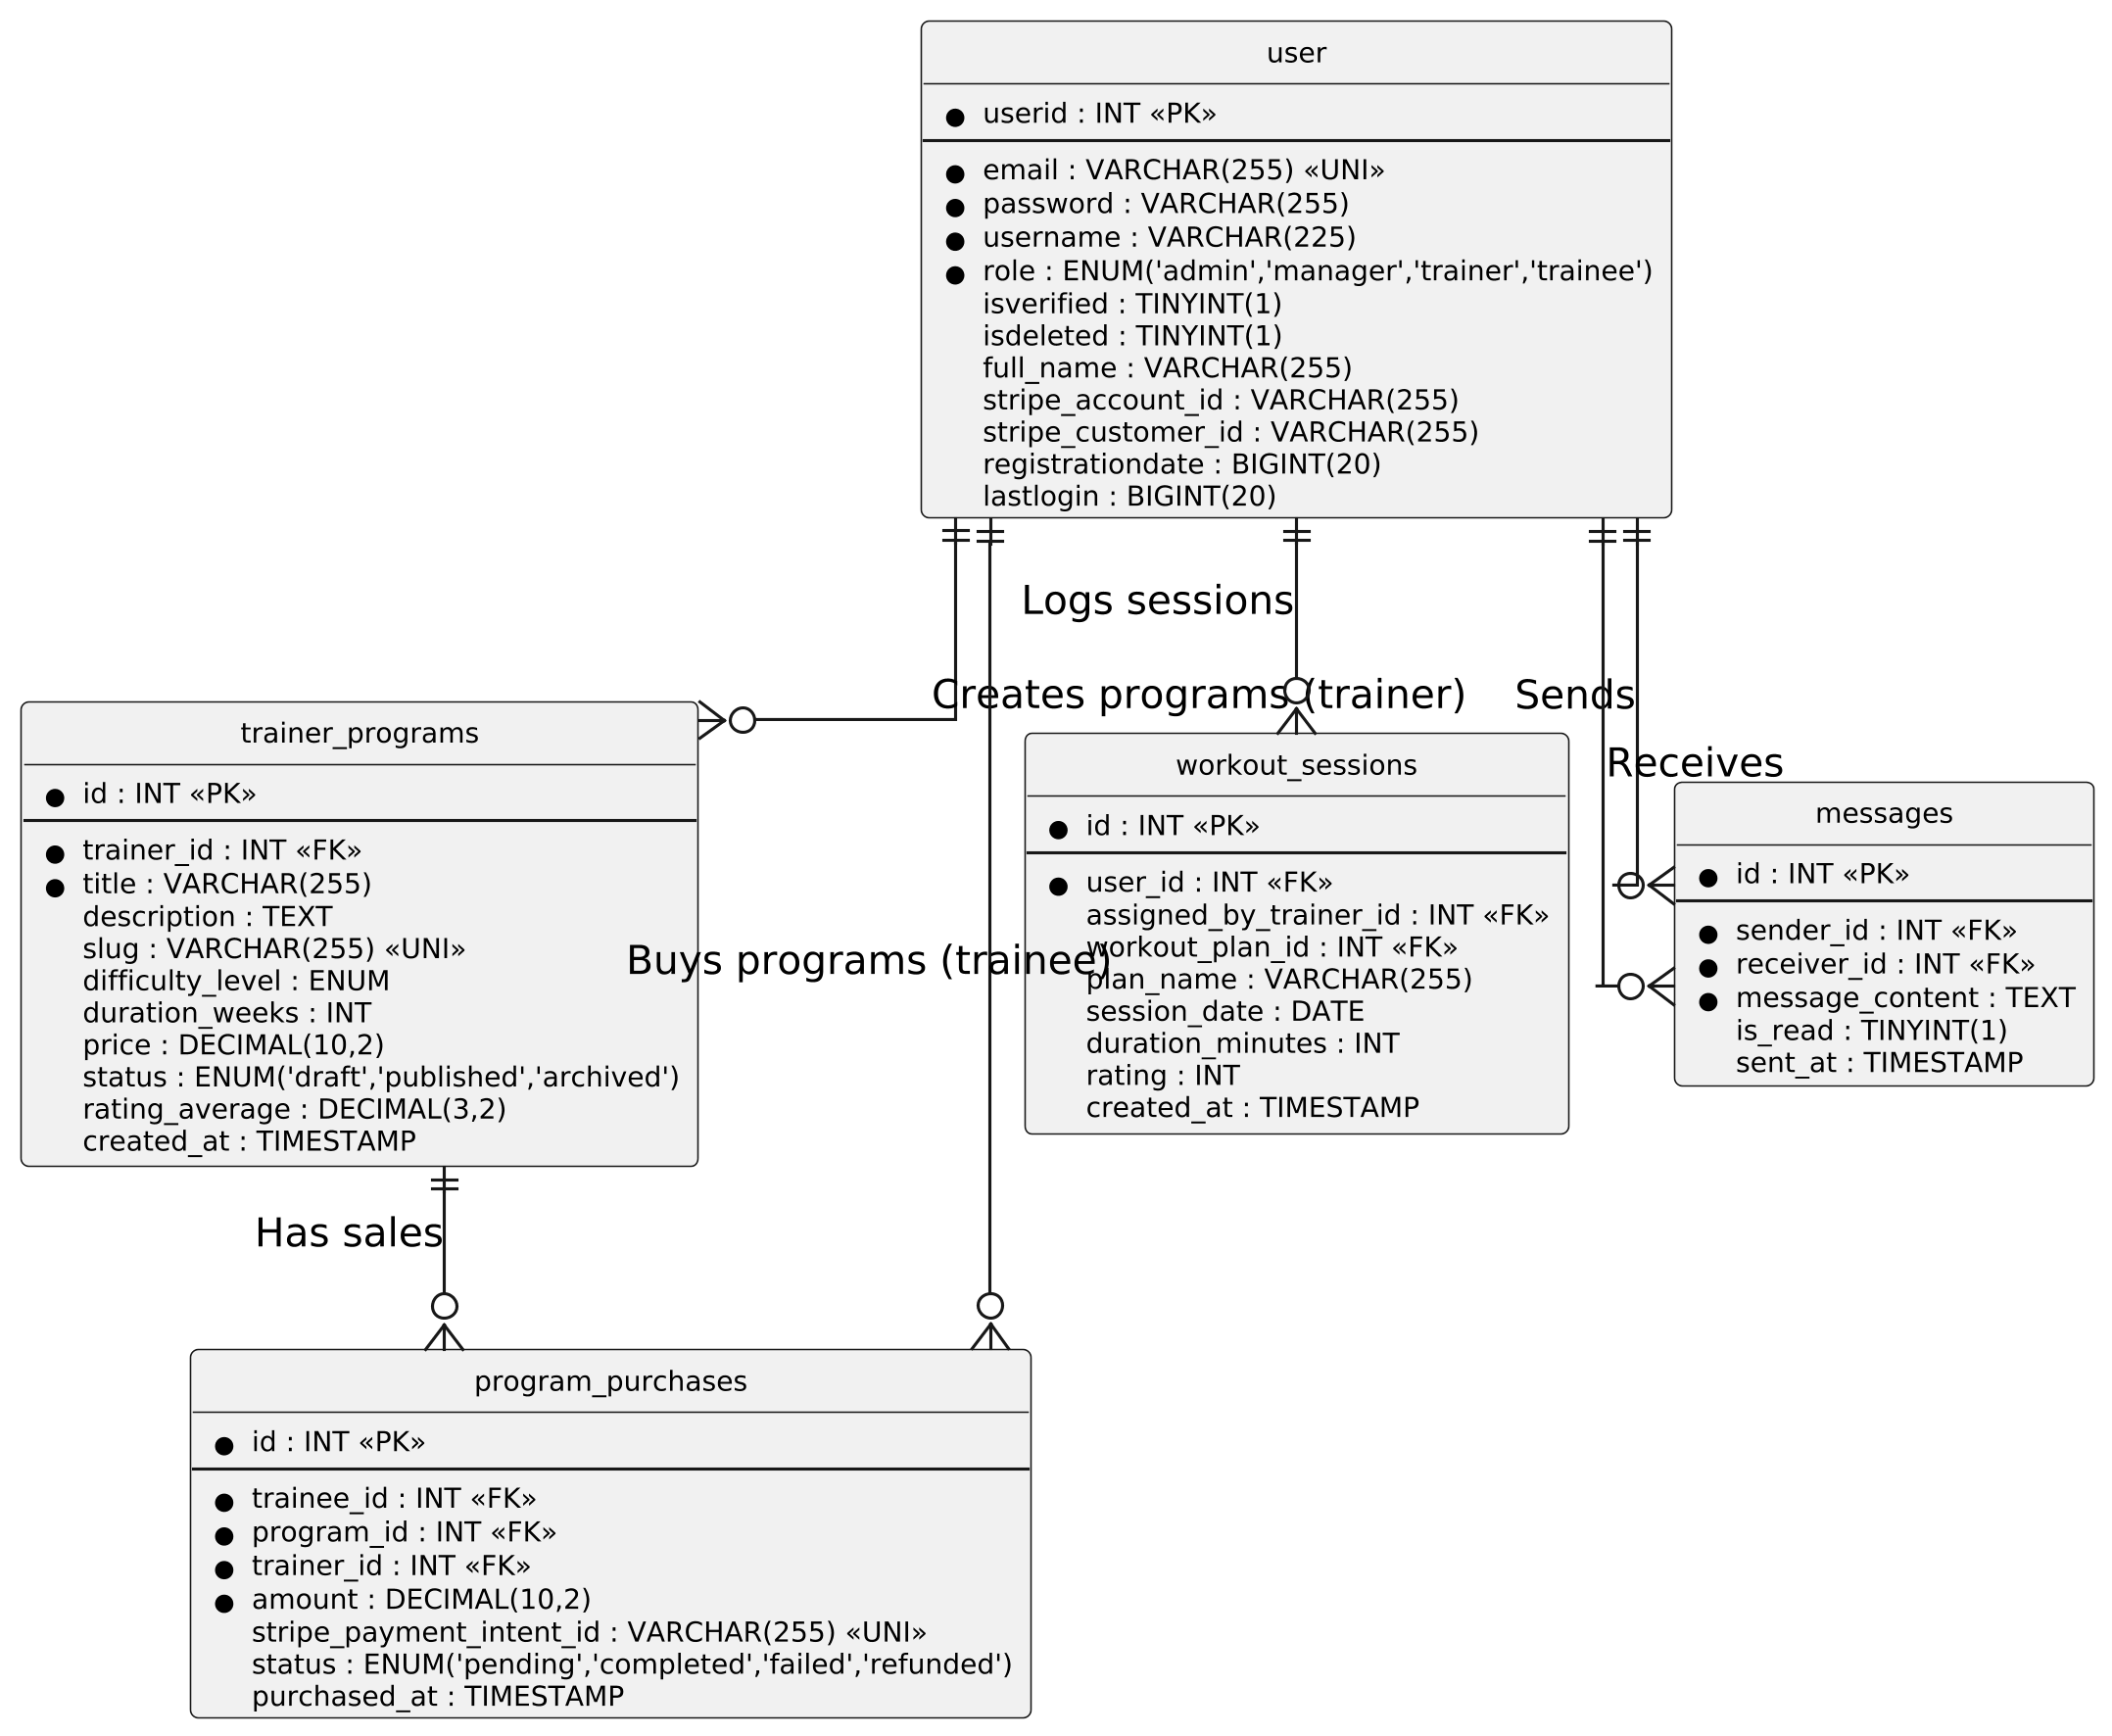
\includegraphics[width=1\textwidth]{db_schema.png}
        \caption{Database Schema ER Diagram}
    \end{figure}

Οι κύριοι πίνακες του συστήματος και οι σχέσεις τους έχουν σχεδιαστεί ώστε να καλύπτουν πλήρως τις ανάγκες διαχείρισης:
\begin{itemize}
    \item \textbf{Πίνακας Users \& Coaches:} Αποθηκεύει στοιχεία προφίλ, επαφών και το ρόλο του χρήστη. Ένας χρήστης συνδέεται με έναν ή περισσότερους προπονητές (σχέση N προς M ή 1 προς N μέσω ενδιάμεσου πίνακα).
    \item \textbf{Πίνακας Workouts \& Nutrition:} Συνδέονται άμεσα με το ID του χρήστη (Foreign Key: User\_ID) στον οποίο έχουν ανατεθεί, καθώς και με το ID του προπονητή που τα δημιούργησε.
    \item \textbf{Πίνακας Progress/Analytics:} Κρατάει ιστορικό σωματικών μετρήσεων του χρήστη ανά ημερομηνία, προσφέροντας data για τα διαγράμματα στο Frontend.
\end{itemize}

* Οι κωδικοί πρόσβασης αποθηκεύονται στη βάση δεδομένων μόνο σε hashed μορφή (π.χ. \textenglish{password\_hash()}), και δεν αποθηκεύονται ποτέ ως απλό κείμενο.

\newpage

% ==========================================
% SECTION 4: ΣΥΝΑΛΛΑΓΕΣ & ΑΠΟΘΗΚΕΥΣΗ (Stripe & Uploads)
% ==========================================
\section{Συναλλαγές και Αποθήκευση Δεδομένων}

\subsection{Ενσωμάτωση Πληρωμών (Stripe API)}
Για την ενοικίαση υπηρεσιών (Hire a coach), το CoachFlow ενσωματώνει το \textbf{Stripe}. 
Όταν ο πελάτης προχωρά σε αγορά, το σύστημα επικοινωνεί μέσω του backend \textenglish{(CreatePaymentIntent.php)} με την πλατφόρμα της Stripe, και επιστρέφει στο Frontend το κατάλληλο \textenglish{client\_secret} για να ολοκληρωθεί η συναλλαγή με ασφάλεια, χωρίς οι πιστωτικές κάρτες να αποθηκεύονται στη δική μας βάση δεδομένων.

\subsection{Αποθήκευση Αρχείων (Media Storage)}
Εικόνες προφίλ των χρηστών, φωτογραφίες προόδου (Progress Photos) και βίντεο/gifs ασκήσεων ενδέχεται να αποθηκεύονται είτε στον φάκελο του server (\textenglish{/frontend/public/assets}) για τα στατικά εικονίδια, είτε σε υπηρεσίες φιλοξενίας όπως το Firebase Storage. Το μέγεθος των αρχείων κατά το ανέβασμα ελέγχεται αυστηρά για να αποφευχθεί η υπερφόρτωση δεδομένων.

\subsection{Επικοινωνία μέσω Email (Mailchimp \& Gmail SMTP)}
Το CoachFlow χρησιμοποιεί δύο συμπληρωματικούς μηχανισμούς για emails:
\begin{itemize}[label=•]
    \item \textbf{Gmail (SMTP):} για transactional emails (signup/verification, reset password, ειδοποιήσεις) που αποστέλλονται από το backend.
    \item \textbf{Mailchimp API:} για διαχείριση audiences/marketing εγγραφών (best-effort), χωρίς να επηρεάζεται η βασική λειτουργία του συστήματος σε περίπτωση προσωρινής αποτυχίας του εξωτερικού service.
\end{itemize}
Τα κλειδιά πρόσβασης και credentials αποθηκεύονται σε μεταβλητές περιβάλλοντος (\textenglish{.env}) και δεν εκτίθενται ποτέ στο frontend.

\newpage

% ==========================================
% SECTION 5: ΑΣΦΑΛΕΙΑ ΚΑΙ SESSIONS
% ==========================================
\section{Ασφάλεια \& Μεταβλητές Sessions (Tokens)}
Το σύστημα χρησιμοποιεί \textbf{HTTP-only PHP sessions} για την εξουσιοδότηση των κλήσεων στο REST API, σε συνδυασμό με \textbf{CSRF protection} και σωστή ρύθμιση \textbf{CORS}. Με αυτό τον τρόπο το frontend (React) μπορεί να είναι decoupled, ενώ το backend παραμένει ασφαλές απέναντι σε επιθέσεις τύπου CSRF/XSS.

\begin{itemize}[label=•]
    \item Κατά το \textenglish{Login}, ο server δημιουργεί session και αποθηκεύει βασικά στοιχεία (π.χ. \textenglish{user\_id} και ρόλο).
    \item Σε κάθε κλήση από το frontend, το session cookie αποστέλλεται αυτόματα (με \textenglish{credentials}) και το backend ελέγχει τα δικαιώματα μέσω \textenglish{Auth.php} (\textenglish{HTTP 401/403} όταν δεν επιτρέπεται πρόσβαση).
    \item Για αποτροπή CSRF, δημιουργείται token στο session και διατίθεται στο frontend (π.χ. cookie \textenglish{XSRF-TOKEN}) ώστε να μπορεί να σταλεί σε headers.
\end{itemize}

Οι πληροφορίες που χρησιμοποιούνται στο session/State είναι:
\begin{itemize}[label=•]
    \item \textenglish{user\_id}
    \item \textenglish{username}
    \item \textenglish{user\_privileges} (\textenglish{trainee / trainer / admin / manager})
    \item \textenglish{logged\_in} (boolean flag)
    \item \textenglish{csrf} (server-side CSRF token που συγχρονίζεται και ως cookie \textenglish{XSRF-TOKEN})
\end{itemize}

\end{document}
